\chapterimage{/10/head.jpg} % Chapter heading image
\chapter{Clustering}\label{10:ch}
Con il termine \textit{clustering} si intendono le proprietà di distribuzione della materia su grande scala. Il clustering viene studiato in modo statistico: si utilizzano principalmente la funzione di correlazione (Paragrafo CITAAAA) e la sua trasfomata di Fourier. Entro un volumetto $\d{V_1}$ la probabilità di trovarvi un oggetto è $\d{P_1}=\overline{n}\d{V_1}$, dove $\overline{n}$ è l densità media di oggetti. La probabilità congiunta di avere un oggetto in due generici volumi, nel caso in cui le singole probabilità siano completamente indipendenti, vale: $\d{P}_{12}=\overline{n}^2 \d{V_1}\d{V_2}$. L'eccesso o il difetto di probabilità rispetto alla distribuzione casuale che darebbe questo risultato è detta \textbf{funzione di correlazione spaziale a due punti}, $\xi(\vec{r}_{12})$. Assumendo isotropia: $\xi(\vec{r}_{12})=\xi(r)$, pertanto si ha la seguente relazione: 
\begin{equation}
    \d{P}_{12}=\overline{n}^2 \d{V_1}\d{V_2} \left(1+\xi(r)\right)
\end{equation}
Per $\xi = 0$ la distribuzione è uniforme, per $\xi >0$ si parla di \textbf{correlazione} e per $\xi <0$ di \textbf{anti-correlazione}. La funzione di correlazione era già stata definita nel caso continuo come correlazione fra il campo $\delta$ e sé stesso in dui punti distanti $r$: $\xi (r)=\langle \delta (x)\delta(x+r) \rangle $. L'uguaglianza tra le due definizioni si può dimostrare facilemente assumendo che tutte le particelle dell'universo abbiano massa uguale. 

Facendo uso del teorema di Bayes si può riscrivere in generale:
\begin{equation}
    \d{P_{12}}= \d{P}(1,2) = \d{P}(1) \d{P}(2|1)\quad \rightarrow \quad \d{P}(2|1)=\overbar{n}\d{V_2}\left(1+\xi(r)\right)
\end{equation}
ossia la probabilità di avere contemporaneamente le condizioni 1 e 2 (rispettivamente un oggetto in $\d{V}_1$ e un oggetto in $\d{V}_2$) è data dalla probabilità di avere 1 moltiplicata per la probabilità (condizionata) di avere 2 dato 1. Da questo è possibile calcolare il numero medio di oggetti entro una sfera centrata su un oggetto dato (e.g. galassie attorno a noi):
\begin{equation}
    \langle N(<r) \rangle =\int \d{P}(2|1) = \frac{4}{3}\pi R^3 \overbar{n} + 4\pi \overbar{n} \int_0^r \d{r'}r'^2 \xi (r') \label{eq10:nummedioentrosfera}
\end{equation}
dove il secondo termine è quello che rappresenta la deviazione dalla distribuzione aspettata data una densità media e un volume. Osservativamente si è visto che:
$$
\xi(r)\propto \left(\frac{r}{r_0}\right)^{-\gamma} \qquad \xrightarrow[z=0]{} \qquad \xi(r)\propto \left(\frac{r}{5\; Mpc/h}\right)^{-1.8}
$$
dove $r_0$ è detta \textbf{lunghezza di correlazione}. Quindi la probabilità di avere un eccesso di coppie su piccola scala è più grande che su grande scala (la tendenza delle galassie è quella di stare vicine vicine). Questa relazione non può continuare per $r\to \infty$, altrimenti il secondo termine dell'Eq. \ref{eq10:nummedioentrosfera} divergerebbe e non si ritroverebbe la densità media dell'universo. Affiché l'integrali si annulli, ci deve essere un punto in cui la funzione di correlazione diventi negativa. Però non può assumere qualsivoglia valore, la proprietà e definita positiva o al più nulla, quindi:
$$
-1 < \xi(r) < +\infty
$$
In ogni caso il valore di $\xi$ tende a $0$ molto velocemente, è difficile da misurare.

Un'alternativa è utilizzare il cosiddetto \textit{conteggio in celle}. In pratica si divide l'universo in tanti piccoli volumi contenenti al più un oggetto. Il numero medio di oggetti entro il volumetto $i$ sarà: $\langle n_i\rangle = \langle n_i^2\rangle = ... =\langle n_i^n\rangle$.
Il numero medio di oggetti entro una sfera centrata su un oggetto a caso nell'universo vale:
\begin{equation}
    \langle N\rangle_V = \int \d{P}(1) \quad \to \quad \Sigma_i \langle n_i\rangle = \overbar{n}V
\end{equation}
Calcolando anche il momento di ordine 2 è possibile ricavare la varianza dei conteggi $\mu_2= \langle N^2 \rangle - \langle N \rangle^2 $:
\begin{equation}
    \langle N^2\rangle_V := \langle\Sigma n_i\; \Sigma n_j \rangle =\overbar{n}V+ \overbar{n}^2V^2 + \overbar{n}^2\int \d{V_1}\d{V_2}\xi_{12} \quad \to \quad \mu_2 = \overbar{n}V+ \overbar{n}^2\int \d{V_1}\d{V_2}\xi_{12}
\end{equation}
Il termine $\overbar{n}V$ è detto \textbf{shot noise} e prescinde dal clustering, che è invece quantificato dall'integrale da cui è possibile fare misure significative su scale molto grandi. La varianza è aumentata dal termine di shot noise a causa della discretezza degli oggetti (un valore di $3.5$ oggetti non è ammissibile). Definendo il contrasto di densità numerica: $\Delta = N - \langle N \rangle / \langle N \rangle$ si può notare che $ \langle \Delta^2 \rangle \propto (\overbar{n}V)^{-1}_{shot}+ V^{-2}\int \d{V_1}\d{V_2}\xi_{12}$, quindi è meglio lavorare su grandi volumi altrimenti il termine di shot noise diventa elevato.
In conclusione, anziché misurare direttamente $\xi$ si preferisce utilizzare i conteggi in sfere poiché il termine da cui si stima, essendo integrato su grandi volumi, diventa più significativo.

\vspace{1em}
Come in tutte le cose della vita alla fine ci si prende gusto e si definisce la \textbf{funzione di correlazione a tre punti}. Questa quantità è necessaria per studiare le distribuzioni non più gaussiane (come per il regime non lineare) aggiungendo informazioni su eventuali direzioni privilegiate. È definita tramite la relazione:
\begin{equation}
    \d{P(1,2,3)}=\d{^3 P}= \overbar{n}^3 \d{V_1}\d{V_2}\d{V_3}\left(1+\xi_3 (r_{12}, r_{13},r_{23})\right)
\end{equation}
con la condizione ovvia $\vec{r}_{12}+ \vec{r}_{13}+\vec{r}_{23}=0$, le variabili da cui dipende $\xi_3$ sono in realtà due. 
\begin{equation}
    \xi_3 (r_{12}, r_{13}, r_{23}) = \xi_2(r_{12}) + \xi_2(r_{13}) + \xi_2(r_{23})+\xi_3^{connessa} (r_{12}, r_{13}, r_{23})
\end{equation}
L'eccesso di probabilità di trovare un tripletto è artificialmente aumentata dal fatto di avere già una coppia, pertanto questi contributi vanno aggiunti al puro eccesso di trovarne solo 3 (\textit{connessa}). Sappiate che avendo $n$ punti, l'unico modo univoco per definire le proprietà della loro distribuzione è conoscere tutti gli $n-1$-esimi momenti. In cosmologia la prima misura di non gaussianità è stata fatta misurando $\Delta^3$ con  $\xi_3$, al massimo ora si arriva a $\Delta^4$ con  $\xi_4$.

\section{Funzione di Correlazione Angolare}
Le stesse quantità appena definite possono essere proiettate angolarmente sul cielo. La misura del redshift è infatti un'approssimazione della distanza vera degli oggetti, che si muovono rispetto al flusso di Hubble con una velocità peculiare $v_{pec}$ difficilmente isolabile. Utilizzare il redshift come terza dimensione ``sporcherebbe'' l'informazione sulla distribuzione degli oggetti. La \textit{funzione di correlazione a due punti angolare} viene così definita:
\begin{equation}
    \d{P}=n_\Omega^2 \d{\Omega_1}\d{\Omega_2}\left( 1+W(\theta)\right)
\end{equation}
dove $\d{\Omega_1}\d{\Omega_2}$ sono piccoli angoli solidi nel cielo che distano $\theta$. In questo modo non ci si sporca le mani con la distanza. Lo stesso approccio è stato utilizzato ai tempi di Peebles (anni '80) quando si avevano solo survey fotometriche e scarsa informazione spettroscopica sui redshift. Per $z=0$ la funzione di correlazione fittata sui dati $\xi(r)$ assume un'andamento del tipo:
$$
W(\theta)\propto \left(\frac{\theta}{\theta_0}\right)^{-0.8}
$$
ossia, proiettandola, viene resa più uniforme. In realtà, esiste una relazione formale per ottenere la distribuzione angolare data una distribuzione spaziale, l'\textbf{equazione di Limber}. Per ottenerla, si considerano la funzione di luminosità $\phi (L) \d{L}$ e il suo legame con la funzione di magnitudine $\psi (M) \d{M}$:
\begin{equation}
    \phi (L) = \left(\frac{L}{L_*}\right)^{-\alpha}e^{-L/L_*} \qquad\qquad \phi (L) \d{L}=\psi (M) \d{M}
\end{equation}
La probabilità di avere in un volumetto una galassia di data magnitudine è: $\d{P}=\psi (M) \d{M}\d{V}$, la funzione di correlazione a due punti viene formalizzata nella forma:
\begin{equation}
    \d{^2P}=\d{M_1}\d{M_2}\d{V_1}\d{V_2} \left(\psi (M_1)\psi (M_2) + G(M_1, M_2, r_{12})\right)
\end{equation}
Notare la differenza ripetto al capitolo precedente. A questo punto si fanno due assunzioni importanti:
\begin{enumerate}
    \item La dipendenza tra magnitudine e distanza è separabile: $G(M_1, M_2, r_{12})=\psi (M_1)\psi (M_2)\xi (r_{12})$. Ora si che la parentesi può tornare: $(1+\xi (r_{12}))$, anche se i dati osservativi non sono molto contenti (soprattutto negli ambienti densi);
    \item Tutte le galassie hanno uguale luminosità $L_*$ (e magnitudine $M_*$): il flusso limite della survey definisce quindi la distanza limite $D_*$ degli oggetti campionati ($D_{Mpc}=10^{0.2(m-M)-5}$);
    \item L'osservazione avviene su angoli piccoli per evitare problemi di curvatura della volta celeste: $r=D_*\sin x \approx D_* x$ ($r$ è la distanza relativa tra due oggetti osservati, $x$ è l'angolo che formano in cielo e $D_*$ è la distanza limite da noi Disgraziati!).
\end{enumerate}
Il numero di galassie medio entro un angolo solido si può quindi scrivere:
\begin{equation}
    n_\Omega = \int^\infty _0 \d{^3r}\int_{-\infty}^{+\infty}\d{M}\psi (M) f(D_*-D) \doteq D_*^3 \int_0^\infty \d{x}\; x^2 \; \psi(x)
\end{equation}
dove $f(D_*-D)$ è una funzione di selezione pari a $1$ se l'argomento è positivo (oggetti entro la distanza imposta dal flusso limite), $0$ altrimenti (nella realtà la transizione non è così netta). In questo modo data una $x$ si scartano tutti gli oggetti che non hanno più la magnitudine tale da essere osservati. Il secondo integrale è poi inglobato in una funzione solo dipendente da $x$, $\psi(x)$. La funzione di correlazione angolare diventa:
\begin{equation}
    \d{^2P}=D_*^6 \int_0^\infty \d{x_1}\; x_1^2 \; \psi(x_1) \int_0^\infty \d{x_2}\; x_2^2 \; \psi(x_2) \left(1+\xi(r_{12})\right)\d{\Omega_1}\d{\Omega_2}
\end{equation}
dove $r_{12}^2=D_*^2 (x_1^2+x_2^2-2x_1x_2\cos \theta_{12})$. Infine, introducendo le quantità: $x=(x_1+x_2)/2$ e $y=(x_1-x_2)/(x\theta_{12})$ si ottiene la fantastica formula:
\begin{equation}
    W(\theta_{12})=\theta_{12}\frac{\int_0^\infty \psi^2(x)x^5\d{x^5} \int_{-\infty}^{+\infty}\xi(D_*\theta_{12}\sqrt{1+y^2}\d{y})}{\left[\int_0^\infty \psi(x)x^2\d{x} \right]}
\end{equation}
detta \textit{equazione di Limber}. Così come la dispersione di velocità delle stelle nelle galassie, i profili di densità e temperatura dei cluster, il lensing e cose di queso tipo... l'equazione può essere utilizzata in due modi:
\begin{itemize}
    \item Assumendo un modello teorico che produce una distribuzione 3D $\xi$ e utilizzandola direttamente per ottenere il $W$ aspettato da confrontare con le osservazioni;
    \item (come si fa di solito) Deproiettando la $W$ osservata attraverso l'equazione invertita.
\end{itemize}
Per due cataloghi con profondità $D_*'\neq D_*$ (magnitudine limite diversa) la funzione di correlazione scala come:
\begin{equation*}
    W'\left(\theta_{12}=\frac{D_*}{D_*'}\theta_{12}'\right)=\frac{D_*}{D_*'}\; W(\theta_{12})
\end{equation*}
ossia, più è profondo il catalogo, meno è clusterata la funzione di correlazione (si omogenizza la distribuzione). In ogni modo, si mantiene l'andamento di $W$ per caloghi di profondità diverse. Come già anticipato, per $\xi \propto r^{-\gamma}$ si ottiene $W\propto \theta^{-\gamma +1}$.

\section{Risultati osservativi}
Per conoscere la distribuzione di materia dell'universo, si può studiare come varia il numero di oggetti al variare del raggio entro cui sono contenuti. Assumendo raggi sufficientemente grandi, la densità media dell'universo tende a zero e l'Equazione \ref{eq10:nummedioentrosfera} diventa:
\begin{equation}
    \langle N(<r)\rangle \propto \int \xi(r) r^2\; \d{r} \qquad \xrightarrow[z=0]{obs} \qquad \langle N(<r)\rangle \propto r^{1.2}
\end{equation}
Le osservazioni locali suggeriscono un andamento con il raggio elevato alla $\sim 1.2$. Per una distribuzione della materia sferica, planare e monodimensionale (filamento), l'esponente dovrebbe essere rispettivamente: $3$, $2$ e $1$. Questo suggerisce che gli oggetti sono distribuiti prevalentemente su filamenti e su piani. In generale:
\begin{equation}
    \langle N(<r)\rangle \propto r^{3-\gamma}
\end{equation}
dove il valore $3-\gamma$ viene detto indice frattale. In base a quanto ricavato, l'universo si dovrebbe auto-riprodurre su tutte le scale. Questo non si verifica perché, come già discusso, la funzione di correlazione deve diventare negativa. [È auspicabile che l'universo non sia un frattale, altrimenti tutto quello che si è fatto fino ad ora andrebbe a farsi benedire: in una distribuzione frattale non si può definire una densità media].

\vspace{1em}
Per calcolare praticamente la funzione di correlazione si utilizza la sua stessa definizione: eccesso/difetto di probabilità rispetto una distribuzione completamente casuale di avere una coppia di oggetti a distanza $r$:
\begin{equation}
    1+\xi(r)=\frac{DD(r)}{RR(r)}            
\end{equation}
dove $DD(r)$ è la distanza tra due oggetti veri (\textit{dato-dato}) e $RR(r)$ è la distanza tra due oggetti appartenenti a un catalogo casuale (\textit{random-random}) avente le stesse caratteristiche di quello vero. Vanno considerati problemi di bordo, zone mascherate e differenti esposizioni. Il numero di coppie è normalizzato al numero di oggetti del catalogo, questo perché il random viene costruito con molti più oggetti. Computazionalmente, si ricorre a tecniche numeriche simili a quelle dei codici N-body (CITAAAAA), altrimenti per calcolare tutte le distanze tra $N$ oggetti sarebbero necessarie $N^2$ operazioni. Un altro stimatore utilizzato, meno sensibile ai problemi accennati, è:
\begin{equation}
    1+\xi(r)= \frac{DD\; RR}{D^2R^2}
\end{equation}

Come già discusso, teoricamente si preferisce utilizzare $\mathcal{P}(k)$, che evolve indipendentemente da $k$ nel regime lineare ed è quindi più semplice da trattare. Dal punto di vista operativo è più facile misurare la funzione di correlazione (Fig. \ref{fig10:2pcf}), che formalmente si ottiene dalla FT della $\mathcal{P}(k)$ (dicono la stessa informazione). Così come lo spettro di potenza evolve come $\delta_+^2$, così fa anche $\xi(r)$.

\begin{figure}[H]
    \centering
    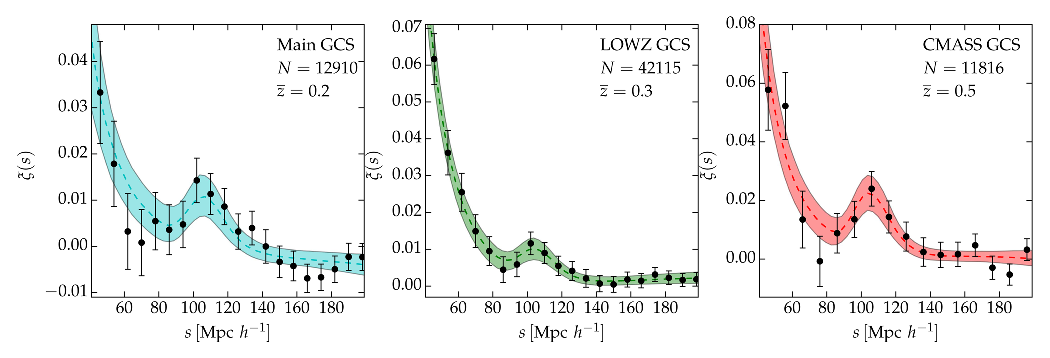
\includegraphics[width=.95 \textwidth]{Pictures/10/2pcf.eps}
    \caption{Funzione di correlazione a due punti (2PCF) nello spazio dei redshift $s$ rispettivamente per i cataloghi: Main-GCS, LOWZ-CGS, CMASS-CGS a reshift medio crescente. L'area shaded è la distribuzione a posteriori derivante dall'analisi MCMC. (From Measuring the distance–redshift relation with the baryon acoustic oscillations of galaxy clusters 2016).}\label{fig10:2pcf}
\end{figure}

\subsection{Bias osservativo}
Gli ammassi di galassie vengono assunti come buoni traccianti della distribuzione della materia a meno di un fattore di bias. In precedenza è stato introdotto come una quantità lineare: $\delta N_g / N_g = b\;  \delta \rho/ \rho$. È chiaro che, per come è stata introdotta, la funzione di correlazione scala come: $b^2$. Al giorno d'oggi si utilizzano modelli non lineari, in cui il bias non dipende semplicemente dalla massa dell'alone host e del redshift (quindi dalla cosmologia). Attraverso il modello dei picchi e del collasso sferico è possibile rendere esplicite queste dipendenze:
\begin{equation}
    b=b(M_{halo}, z) \simeq 1 + \frac{1}{\delta_c} \left(\frac{\delta_c^2}{\sigma_M^2\delta_+^2(z)}-1\right)
\end{equation}
confermate anche da simulazioni N-body e perfezionate da modelli di collasso ellissoidale. Dal momento che $\sigma_M$ decresce con $M$, $b$ è una funzione crescente di $M$; ossia oggetti più massicci tendono ad essere più clusterati (cfr. discorso delle Alpi, teoria dei picchi). Inoltre, il fattore di crescita diminuisce all'aumentare di $z$: i cluster a $z=2$ sono più clusterati di quelli a $z=0$ (sono sovradensità più estreme rispetto al valore medio del campo di densità). La $\xi$ degli ammassi ($r_0^{cluster} \sim 15\div 25$ Mpc/h a $z=0$) è più grande di quella delle galassie ($r_0^{gal} \sim 5$ Mpc/h a $z=0$). Queste sono sporcate dalla microfisica, misurando il clustering degli aloni è possibile porre constraints sulla: cosmologia conoscendo la loro massa, massa assumendo una cosmologia.

Per ragionamenti analoghi, le galassie early type sono più clusterate rispetto alle late type a parità di $z$ e questo è confermato da dati osservativi. 


\subsection{Moti peculiari}
Come già discusso, il redshift non è un buon indicatore della distanza. Questo è dovuto al fatto che le galassie possono avere una velocità peculiare $v_{pec}$ che le dissocia dal flusso di Hubble (e.g. Andromeda rispetto a noi):
$$
v = H(z)d + v_{pec}
$$
questa quantità non è sempre stimabile. L'effetto ha come conseguenza che un oggetto sferico nello spazio reale appare distorto nello spazio dei redshift (Fig. \ref{fig10:bella}). Questo tipo di distorsione è detto \textit{finger of God}. I grandi flussi di materia che collassano verso il centro sono moti \textit{bulk} e anch'essi portano a distorsioni. Si può dimostrare che $\xi(s)$ nello spazio dei redshift è in generale più piatta di $\xi (r)$ nello spazio fisico a piccoli $r$.

\begin{figure}[H]
    \subfloat[]{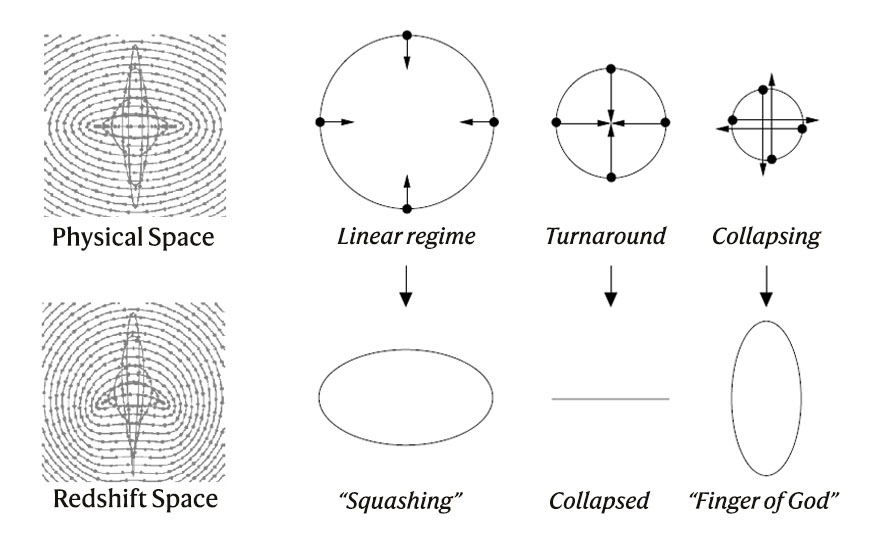
\includegraphics[width=.66\textwidth]{Pictures/10/fog.jpg}}$\;\;$
    \subfloat[]{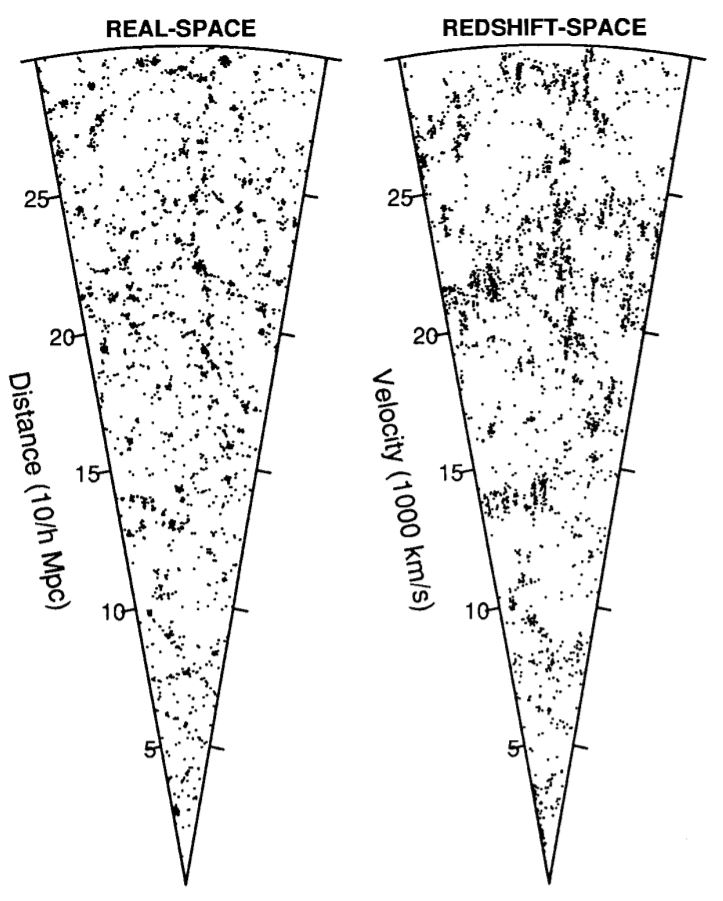
\includegraphics[width=.295\textwidth]{Pictures/10/fogsim.jpg}}
    \caption{(a) Effetto delle velocità peculiari nello spazio dei redshift. L'osservatore è posto in basso. Nell'immagine in alto a sinistra i punti rappresentano diverse galassie: quelli connessi sono galassie che distano in modo uguale dal centro di una sovradensità sferica (ammasso) nello spazio reale. A grande distanza le galassie cadono nel cluster: quelle più vicine a noi appaiono (spazio dei redshift) più distanti. Avvicinandoci alla regione interna virializzata, le velocità di dispersione aumentano e nello spazio dei redshift si forma il \textit{finger of God}.  , $v_{pec} <0$ (From: hneider Astronomy and Cosm CITAAAAS); (b) Fetta di universo simulato nello spazio reale e in quello dei redshift (From: Patron - \textit{The Bull's-Eye Effect: Are Galaxy Walls Observationally Enhanced? CITAAA.}} \label{fig10:bella} 
\end{figure}


Per ovviare a questo problema si può ricorrere alla \textbf{funzione di correlazione proiettata} lungo la linea di vista (è simile a quella angolare). Si assume che il redshift sia una misura esatta della distanza, che viene scomposta in due contributi, perpendicolare e parallelo alla linea di vista: $s^2 =  r_\perp^2 + \pi^2$. È il termine $\pi$ lungo la linea di vista che crea problemi, pertanto si integra su questa dimensione:
\begin{equation}
    W_{proj}(r_\perp ):=\int_0^\infty \xi(r_\perp, \pi)\d{\pi}=2\int_{r_\perp}^\infty\frac{\xi(s)\;\d{s}}{\sqrt{s^2-r_\perp ^2}} 
\end{equation}
dove $1+\xi(r_\perp , \pi)= DD/RR$. Proiettando si perde un po' di informazione, ma rimane soltanto quella pulita.

\vspace{1em}
Alternativamente, si può sfruttare la distorsione come informazione cosmologica. La velocità peculiare è dovuta al fatto che la materia non è distribuita in modo uniforme. Questo è un modo potente per testare la relatività generale nel tempo. Inizialmente si calcola la $W_{proj}$. Se la funzione di correlazione fosse isotropica, nel piano $(r_\perp,\pi)$ si avrebbero dei cerchi perfetti con raggio crescente al diminuire di $W$. Si assume che questa sia la funzione di correlazione nello spazio reale. La componente lungo la linea di vista si osserva invece distorta: schiacciata su grandi scale e \textit{finger of god} su piccole scale (Fig. ). Il primo è un effetto giustificabile e quantificabile dalla teoria lineare:
\begin{equation}
    \xi(s)=\xi(r)\left(1+\frac{2}{3}f+\frac{1}{5}f\right);\qquad f=\frac{\d{\ln \delta_+}}{\d{\ln a}}\simeq \Omega_M^{0.55}+...
\end{equation}
In questo modo è possibile misurare $\Omega_M$ o, meglio ancora, a diversi redshift, verificare la validità della relatività generale. Questo è uno dei test che farà Euclid. Prima questo era rumore, ora è oro. In realtà per le galassie, $f\to f/b$.
\begin{figure}[H]
    \centering
    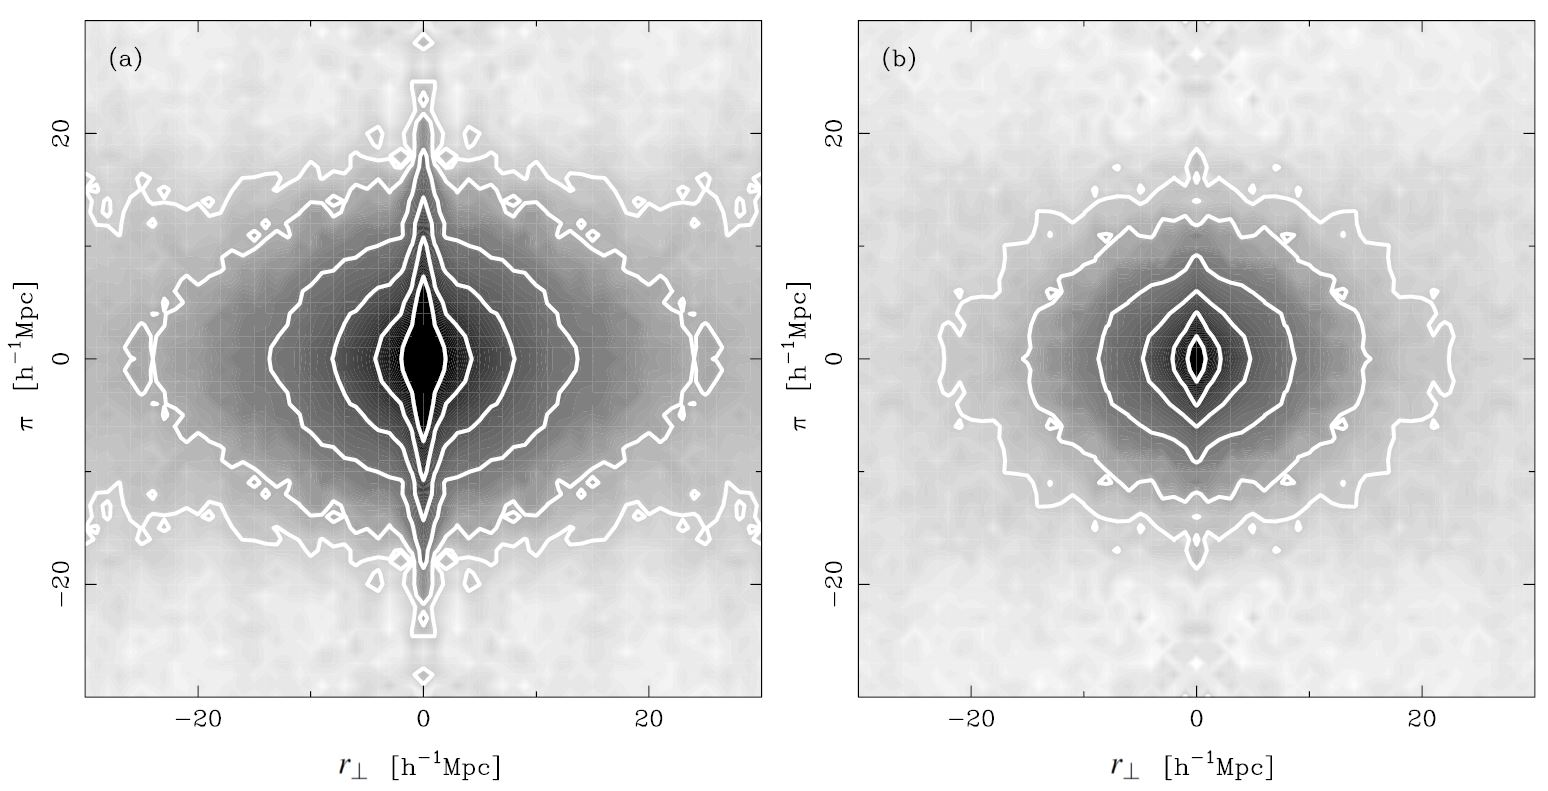
\includegraphics[width=.75 \textwidth]{Pictures/10/apforse.jpg}
    \caption{Funzioni di correlazione proiettate per: galassie quiescienti (sinistra), galassie starforming (destra). Come mai differiscono? Io forse lo so, ma non ve lo dico! (From: The 2dF Galaxy Redshift Survey: galaxy clustering per spectral type CITAAA)}
\end{figure}

\vspace{1em}
Infine, un altro modo di sfruttare questa informazione è tramite il test di \textbf{Alcock-Paczynski}. Per convertire quantità angolari e distanze in coordinate cartesiane bisogna assumere una cosmologia. Quindi il risultato della funzione di correlazione con i metodi visti in precedenza dipende anche dalla cosmologia. In questo caso si fa la procedura opposta: dopo aver modellato via tutte le distorsioni dinamiche possibili (il finger of god è il più difficile), si cerca l'unica cosmologia che restituisce $\xi (r)$ in cerchi perfetti. Questo può essere applicato su tutti gli oggetti di forma nota, e.g. sui vuoti assumendo che siano perfettamente sferici.